\documentclass[dvisvgm,multi=true]{standalone}
\usepackage{mathmlcoresvg}
\begin{document}
%<figcaption><span>Figure 22: </span>Box model for the <code>msubsup</code> element</figcaption>
  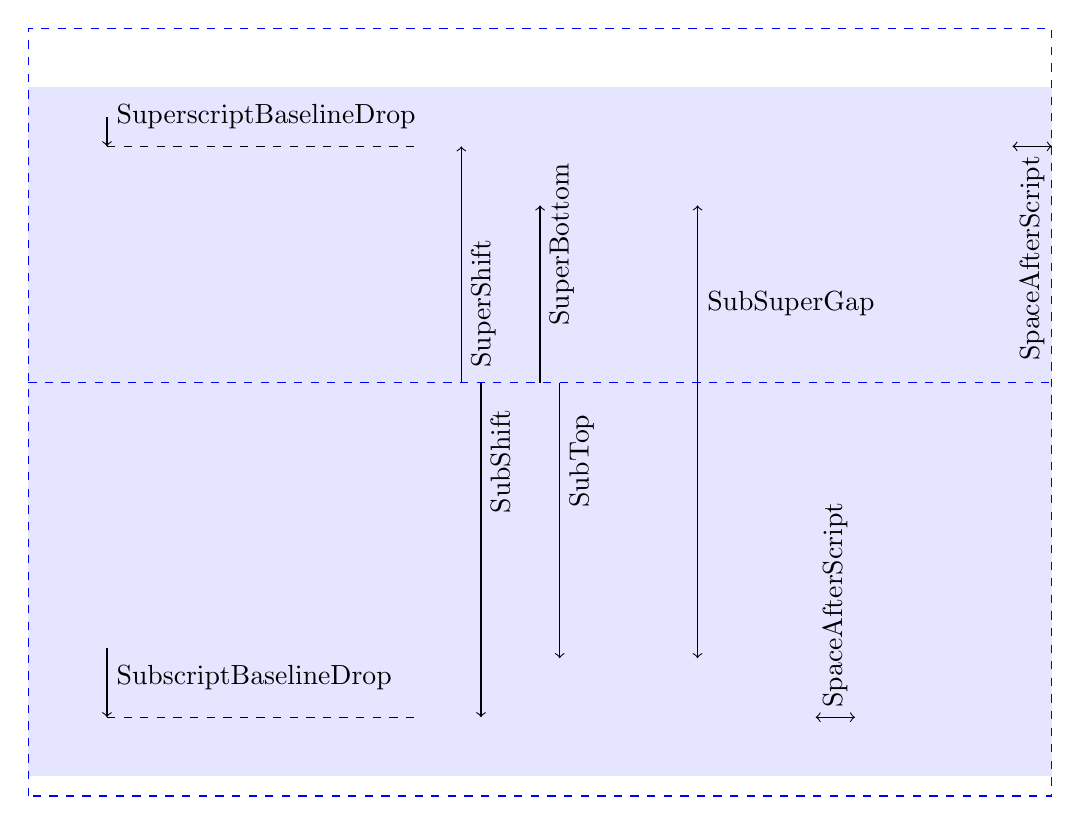
\begin{tikzpicture}[yscale=-1]

  \fill[blue!10](0,5) rectangle (13,-3.75);

  \MathMLBox{0}{0}{1}{2.25}{red};

  \MathMLBox{5}{-3}{1.5}{.5}{green};

  \draw[dashed,blue](0,5.25) rectangle(13,-4.5)
  (0,0)--(13,0);

  \draw[->] (5.5,0) -- (5.5,-1)node[below,rotate=90]{SuperShift} -- (5.5,-3);

  \draw[->] (6.5,0) -- (6.5,-1.75)node[below,rotate=90]{SuperBottom} -- (6.5,-2.25);

  \draw[<->] (12.5,-3) -- (12.75,-3)node[left,rotate=90]{SpaceAfterScript} -- (13,-3);

  \MathMLBox{5}{4.25}{1}{.5}{green};

   \draw[->] (5.75,0) -- (5.75,1)node[below,rotate=90]{SubShift} -- (5.75,4.25);

  \draw[->] (6.75,0) -- (6.75,1)node[below,rotate=90]{SubTop} -- (6.75,3.5);

  \draw[<->] (10,4.25) -- (10.25,4.25)node[right,rotate=90]{SpaceAfterScript} -- (10.5,4.25);

   \draw[<->] (8.5,-2.25) -- (8.5,-1)node[right]{SubSuperGap} -- (8.5,3.5);

   \draw[->] (1,-3.375) node[right]{SuperscriptBaselineDrop} -- (1,-3);
   \draw[dashed] (1,-3) -- (5,-3);

   \draw[->] (1,3.375) -- (1,3.75) node[right]{SubscriptBaselineDrop} -- (1,4.25);
   \draw[dashed] (1,4.25) -- (5,4.25);
\end{tikzpicture}

\end{document}
